\chapter{Návrh}

V této kapitole se budeme věnovat návrhu knihovny na automatizaci a jejím funkčním požadavkům.

\section{Zařízení}
Jak již z předchozích částí práce plyne, zařízení, která využívají průmyslovou komunikaci, jsou velmi specifická. Tato zařízení běží na speciálně vyvinutém hardwaru. Zařízení budou připojena za pomocí Ethernetu k zařízení, na kterém poběží testovací knihovna a další služby k řízení testování. Zařízení, na kterém poběží testovací služba, poběží na systému Windows od společnosti Microsoft, kvůli dobré interoperabilitě se serverem Azure DevOps. Zároveň jsou systémy od společnosti Microsoft preferovány společností Siemens. 

\section{Komunikace}
Komunikace mezi participanty bude fungovat na principu TCP/IP připojení. Zároveň zprávy, které budou mezi službou a participanty vyměňovány, budou mít stanovenou strukturu. Jedna zpráva bude obsahovat délku zprávy, typ zprávy a poté data zprávy. Data zprávy se budou odvíjet od typu zprávy. Existují i situace, kdy zpráva žádná data obsahovat nebude, k přenesení informace tedy bude stačit pouze typ zprávy. Složení zprávy lze vidět na obrázku \ref{fig:message}. 

\begin{figure}[htbp]
    \centering 
    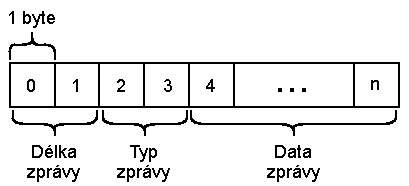
\includegraphics{assets/img/message.pdf}
    \caption{Diagram struktury jedné zprávy}
    \label{fig:message}
\end{figure}


\section{Služba}
Ve vyvíjené knihovně bude jádrem k řízení testování služba, která se bude starat o běh testu. Služba v počáteční fázi vytvoří připojení se všemi fyzickými participanty testu. Po připojení určitého počtu očekávaných participantů započne samotné testování. Služba bude spouštět testy a během testu bude synchronizovat stádia testování mezi všemi participanty testu. Následně po běhu testu vyhodnotí úspěšnost testu na základě dat, které obdrží od participantů. 


\section{Virtuální participant}
Knihovna zároveň bude obsahovat tzv. virtuálního participanta. Toto zařízení bude sloužit k simulaci protistrany u testování fyzického zařízení. Je to volitelný participant. Simulováním participanta snižujeme hardwarové nároky na testování, což vede ke snížení nákladů. Tato zařízení se budou moct připojovat v průběhu testovací běhu, v závislosti a potřeby jednotlivých testů.


\section{Rozhraní pro testované zařízení}
Součástí bude taktéž bude rozhraní, pro implementaci zařízení, které bude testováno. Toto rozhraní bude mít jasně definovanou  strukturu, ale zároveň bude co nejjednodušší pro co nejrychlejší implementaci na nově testovaném zařízení. Toto rozhraní bude potom využito pro řízení běhu testu na testovaném zařízení.

Součástí rozhraní bude i rozhraní pro jednotlivé testy. To bude obsahovat jednotlivá stádia testování, která budou mezi všemi zařízeními synchronizovány. Tyto stádia budou, v tom pořadí:
\begin{enumerate}
    \item Příprava na testování
    \item Samotné testování
    \item Úklid po testu
\end{enumerate}


\section{Propojení së serverem Azure DevOps}
Propojení se serverem Azure DevOps bude vytvořeno za pomocí testovacího frameworku MSTest. Tento framework umožní skrz server Azure DevOps automaticky spouštět testy. Zároveň poté bude možné jednotlivé testy registrovat na serveru. 


